\documentclass[14pt, a4paper]{article}
\usepackage[T2A]{fontenc}
\usepackage[utf8]{inputenc}
\usepackage[russian]{babel}
\usepackage[left=3cm, right=1.5cm, top=2cm, bottom=2cm]{geometry}
\usepackage{indentfirst}
\usepackage{microtype}
\usepackage{array}
\usepackage{xcolor}
% \usepackage{times}
\usepackage{tempora}
\usepackage{ulem}
\usepackage{setspace}
\usepackage{amsmath}
\usepackage{booktabs}
\usepackage{graphicx}
\usepackage{float}
\usepackage{listings}
\graphicspath{{reports/figures/}{figures/}}
\lstset{basicstyle=\ttfamily\small, breaklines=true, columns=fullflexible, frame=single, keepspaces=true}
\pagestyle{empty}

\makeatletter
\renewcommand\section{\@startsection {section}{1}{\parindent}%
  {-3.5ex \@plus -1ex \@minus -.2ex}%
  {0.5ex}%
  {\normalfont\Large\bfseries}}
\renewcommand\tableofcontents{%
  \begin{center}\Large\bfseries\contentsname\end{center}%
  \@starttoc{toc}%
}
\renewcommand*\l@section{\@dottedtocline{1}{0em}{1.5em}}
\makeatother

\begin{document}
\onehalfspacing

\begin{center}
    \textbf{ФЕДЕРАЛЬНОЕ ГОСУДАРСТВЕННОЕ АВТОНОМНОЕ ОБРАЗОВАТЕЛЬНОЕ} \\
    \textbf{УЧРЕЖДЕНИЕ ВЫСШЕГО ОБРАЗОВАНИЯ} \\
    \textbf{«МОСКОВСКИЙ АВИАЦИОННЫЙ ИНСТИТУТ} \\
    \textbf{(НАЦИОНАЛЬНЫЙ ИССЛЕДОВАТЕЛЬСКИЙ УНИВЕРСИТЕТ)»}
\end{center}

\begin{center}
    \bfseries Институт №8 «Компьютерные науки и \\
    \bfseries прикладная математика» \\
    \bfseries Кафедра 806 «Вычислительная математика \\
    \bfseries и программирование»
\end{center}

\vspace{3cm}

\begin{center}
    \Large\bfseries Отчет \\
    \vspace{0.5cm}
    \mdseries по лабораторной работе №2.2
\end{center}

\vfill

\noindent
\hfill
\begin{tabular}{ll}
Группа:       & М8О-307Б-21 \\
Студент:      & М. С. Ивченко \\
Преподаватель:& доц. В. В. Киндинова \\
Оценка:       & \underline{\makebox[3cm][c]{}} \\ [0.2cm]
Дата:         & \underline{\makebox[3cm][c]{}}
\end{tabular}

\vfill

\begin{center}
    Москва \\
    2026
\end{center}

\newpage

\setcounter{tocdepth}{2}
\tableofcontents
\newpage

\section*{Тема}
\addcontentsline{toc}{section}{Тема}
Цель данной лабораторной работы -- перейти от одного нелинейного уравнения к системам нелинейных уравнений. Работа посвящена построению итерационного процесса для нескольких неизвестных, использованию матрицы Якоби в методе Ньютона и анализу сходимости полученных приближений.

\section*{Задание}
\addcontentsline{toc}{section}{Задание}
Реализовать методы простой итерации и Ньютона решения систем нелинейных уравнений в виде программного кода, задавая в качестве входных данных точность вычислений. С использованием разработанного программного обеспечения решить систему нелинейных уравнений (при наличии нескольких решений найти то из них, в котором значения неизвестных являются положительными); начальное приближение определить графически. Проанализировать зависимость погрешности вычислений от количества итераций.

\section*{Теория}
\addcontentsline{toc}{section}{Теория}
Система нелинейных уравнений записывается в векторном виде
\[
    F(x)=0,\qquad F=(f_1,\ldots,f_n)^T,\quad x=(x_1,\ldots,x_n)^T.
\]
В отличие от одного уравнения, здесь важно выбрать начальную точку в нужной области, потому что система может иметь несколько решений. Графический анализ линий уровня $f_i(x)=0$ помогает определить, где пересекаются кривые и какое начальное приближение приведет к положительному решению.

Метод Ньютона для системы использует многомерную линеаризацию:
\[
    F(x_k+\Delta x)\approx F(x_k)+J(x_k)\Delta x,
\]
где $J(x)$ -- матрица Якоби, составленная из частных производных $j_{ij}=\partial f_i/\partial x_j$. Чтобы новое приближение приблизило систему к нулю, на каждом шаге решается линейная система
\[
    J(x_k)\Delta x_k=-F(x_k), \qquad x_{k+1}=x_k+\Delta x_k,
\]
Если начальная точка достаточно близка к решению, а матрица Якоби невырождена, метод Ньютона обычно сходится квадратично. Главная вычислительная стоимость шага -- решение СЛАУ с матрицей Якоби.

Метод простой итерации задается векторной функцией
\[
    x=\Phi(x), \qquad x_{k+1}=\Phi(x_k).
\]
Достаточное условие сходимости -- сжатие отображения в выбранной области:
\[
    \|\Phi'(x)\|\le q<1.
\]
Здесь $\Phi'(x)$ -- матрица производных итерационной функции. Если условие выполнено, погрешность оценивается по разности соседних векторов:
\[
    \|x^*-x_k\|\le\frac{q}{1-q}\|x_k-x_{k-1}\|.
\]
Остановка итераций выполняется по норме шага $\|x_{k+1}-x_k\|$ и дополнительно проверяется по невязке $\|F(x_k)\|$.

\begin{lstlisting}[language=Python]
f_val = eval_f(x_curr)
J_val = get_jacobian(x_curr)
delta_x = np.linalg.solve(J_val, -f_val)
x_next = x_curr + delta_x
\end{lstlisting}

\section*{Ход лабораторной работы}
\addcontentsline{toc}{section}{Ход лабораторной работы}
Решалась система
\[
\begin{cases}
x_1-\cos x_2-2=0,\\
x_2-\sin x_1-2=0.
\end{cases}
\]
Для метода простой итерации использовалась форма
\[
    x_1=\cos x_2+2,\qquad x_2=\sin x_1+2.
\]
По пересечению кривых начальная область решения выбрана около $[0.8,1.2]\times[2.8,3.2]$.

\begin{figure}[H]
    \centering
    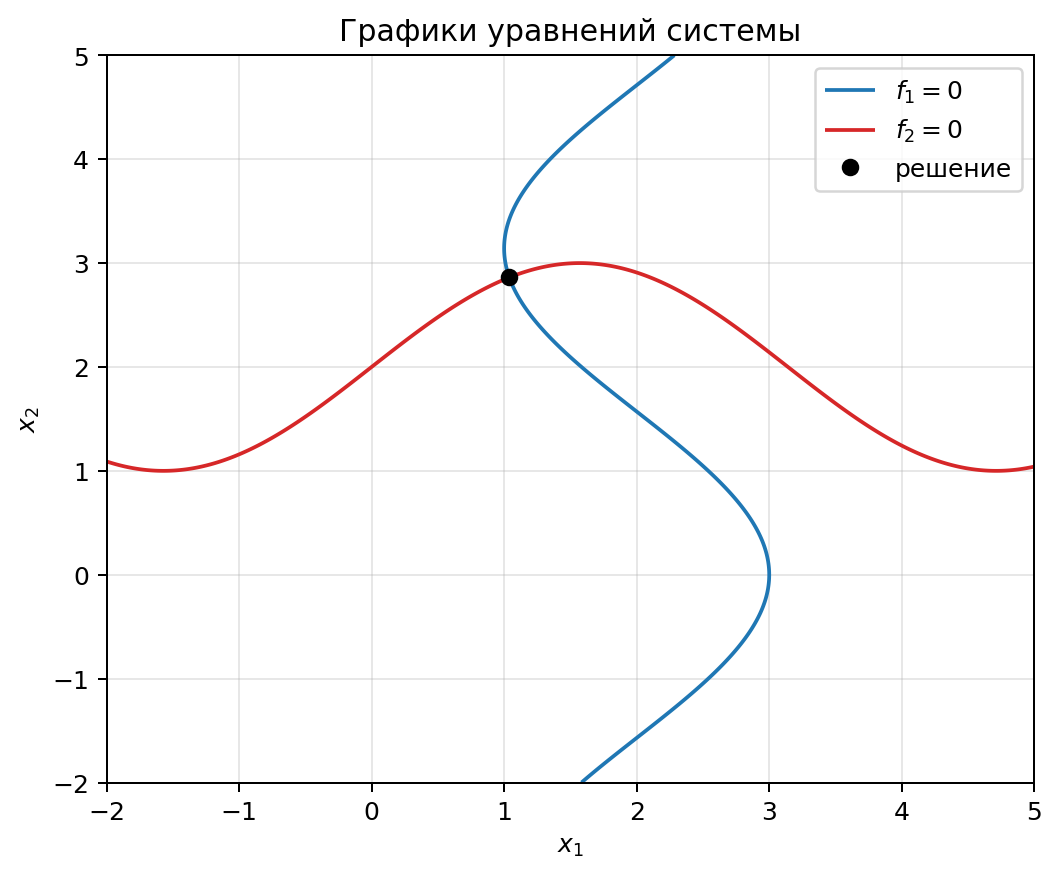
\includegraphics[width=0.86\textwidth]{lab2_2_contours.png}
    \caption{Графическое определение начального приближения для системы.}
\end{figure}

Метод Ньютона из точки $(1,3)$ сошелся за 3 итерации к
\[
    x=(1.03887749,\;2.86183545)^T,
\]
невязка по компонентам не превышает $3.1\cdot10^{-10}$. Метод простой итерации из точки $(1,2)$ сошелся за 13 итераций к $x=(1.03887912,2.86183529)^T$.

\begin{figure}[H]
    \centering
    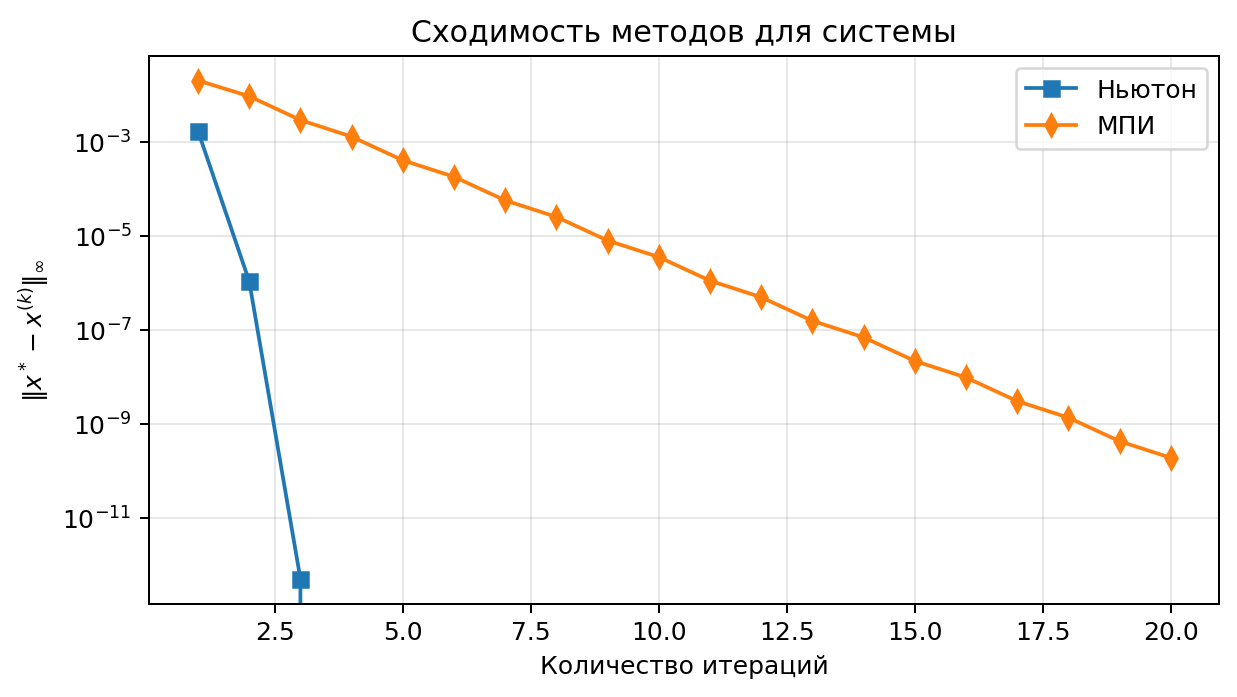
\includegraphics[width=0.86\textwidth]{lab2_2_errors.png}
    \caption{Сравнение скорости сходимости метода Ньютона и простой итерации для системы.}
\end{figure}

\section*{Выводы}
\addcontentsline{toc}{section}{Выводы}
Метод Ньютона заметно быстрее за счет учета якобиана: уже после трех итераций достигается практически эталонное решение. Метод простой итерации также сходится, но требует больше шагов и зависит от выполнения условия сжатия для выбранной $\Phi$.

\end{document}
